% ID: SEL-D0018-BB-E03
% ESTADO: validada. S019. Revisión matemática, didáctica y visual.
\textbf{a) Tangente.}\par\nopagebreak[4]
La pendiente es $f'(1)=-4$. Como $f(1)=3$, la ecuación punto-pendiente es $y-3=-4(x-1)$, es decir, $\boxed{y=-4x+7}$.

\textbf{b) Monotonía y extremos.}\par\nopagebreak[4]
Como $f'(x)=2(x-3)$, la función decrece para $x<3$ y crece para $x>3$. El cambio de signo de negativo a positivo determina un mínimo en $x=3$. Sobre $\mathbb R$ es el mínimo absoluto y no hay máximo.

\textbf{c) Expresión y gráfica.}\par\nopagebreak[4]
Al integrar obtenemos $f(x)=x^2-6x+C$. De $1-6+C=3$ sale $C=8$. Así,
\[
\boxed{f(x)=x^2-6x+8=(x-3)^2-1}.
\]
La parábola tiene vértice $(3,-1)$, eje $x=3$, raíces $2$ y $4$ y ordenada en el origen $8$.
\begin{center}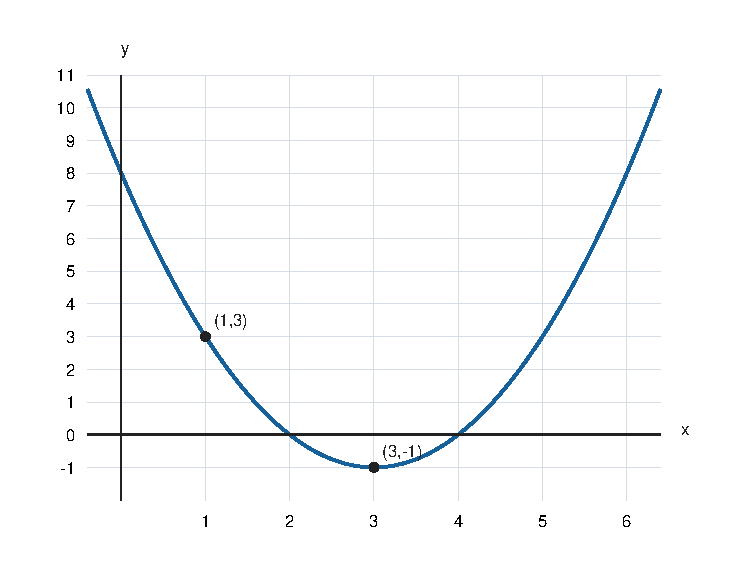
\includegraphics[width=0.51\linewidth]{recursos/figuras/s019-parabola.pdf}\end{center}
